\section{Digital Communication Interface and Readout}
\label{sec:logic_design}


\subsection{Description of the ASIC digital subsystem}
\label{sec:descriptionASIC}


\begin{figure}[H]
    \centering
    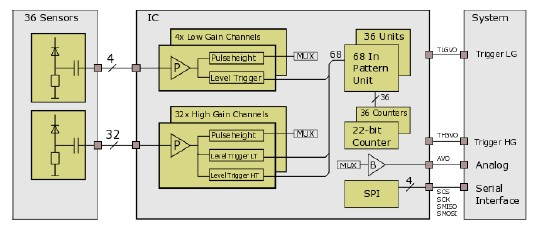
\includegraphics[width=1\textwidth]{ASIC_schematic.jpg}
    \caption[]{Block Diagram Schematic of the ASIC (VATA466/ide3466) (\cite{Meier2016VATA466}) }
    \label{fig:ASIC_schematic}
\end{figure}

\subsubsection{Input Channels}

From the figure above it can be seen that each diode anode is AC-coupled to one input. The ASIC has 4 Low Gain (LG) channels and 32 High Gain (HG) channels, which serve as input from the detector diodes of the directionality sensor. Each channel has one pre-amplifier and an analogue processing for pulse height and level triggers. In the figure below, the channel inputs are depicted on the left side of the scheme.

\begin{figure}[H]
    \centering
    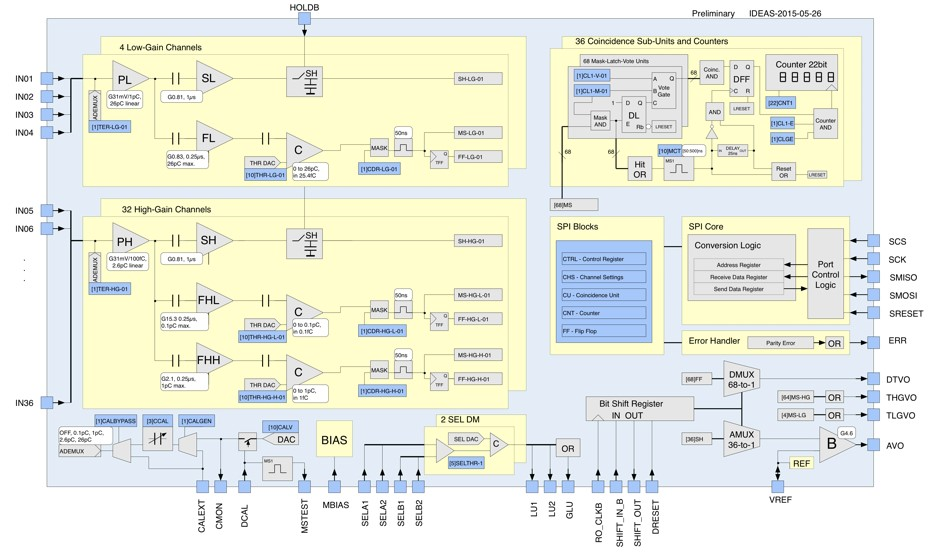
\includegraphics[width=0.9\textwidth]{ASIC_Functional.jpg}
    \caption[]{ASIC functional schematic with I/O (VATA466/ide3466) (\cite{Meier2016VATA466}) }
    \label{fig:ASIC_Functional}
\end{figure}

\subsubsection{Modes of operation}

The ASIC has two modes of operation and each of the modes requires a different approach for the readout. It can be used in the Counting Mode Acquisition (CMA) or Spectroscopic Mode Acquisition (SMA). 
\newline
The CMA is the mode for which the digital hardware was designed. In this mode, the values of a total of 36 registers, which comprise the so-called Coincidence Sub-Unit (CSU) of the ASIC, can be read. The CMU, its registers and configuration principle is described later in this section. The value in each of the registers reflects the number of events that occurred, which fulfill the requirements of any individual out of 36 prior defined coincidences.
\newline
The following steps are required to run this mode successfully:





\begin{itemize}
\item Configuration of the analogue channel thresholds through channel configuration registers

\item Configuration of the coincidence units with channel trigger coincidence and anti-coincidence through Coincidence Sub-Unit configuration registers
\item Periodic read-out of the coincidence counter registers

\end{itemize}

The SMA mode will only be explained briefly in this report.
Its objective is to recreate the shape of the detected
pulses. The pulses which are registered in the input
channels can be transformed to 36 analogue values by a slow
shaper and can be later read out serially with the help of
an analogue multiplexer (36-to-1 AMUX) that is controlled
by the RO\_CLKB, SHIFT\_IN\_B and DRESET inputs as seen in
\ref{fig:ASIC_Functional}, the signal SHIFT\_OUT
indicates when the operation is finished.

The parts of the subsystem will be described with regards to the counting mode acquisition. 

\subsubsection{Registers}

The registers in the ASIC have a length of 22 bit, each register can be mapped to by a 9-bit address.

\subsubsection{Channel Thresholds}

Each of the low gain channels has one and each of the high gain channels has two channel configuration registers associated with them. The values in the registers determine the charge threshold for their respective comparator. In the ASIC, a digital pulse is generated when the amount of charge that is generated at the respective input channel exceeds the value defined in the comparator. One threshold can be set for the low gain channels and two thresholds can be set for the high-gain channels, hence the need for 2 channel configuration registers for the HG channels.

\subsubsection{Coincidence Unit}

There are in total 36 CSUs. Each sub-unit is associated with 7 CSU configuration registers, that collectively define a coincidence. A coincidence is essentially a combination of digital pulses that were triggered based on the set channel thresholds. In the configuration registers, it can be defined if a channel shall be considered in a coincidence through a mask bit and whether it must have triggered through a coincidence / anti-coincidence (C/Ac) bit. If the triggered digital pulses fulfill the coincidence requirements, the specific CSU’s counter is increased by one. The reason we need 7 configuration registers for each CSU is the following: 
\newline
There are four LG channels, each with one (C/Ac) bit and one mask bit. And 32 HG channels, each with two thresholds and each of the thresholds with one (C/Ac) bit and one mask bit).

\begin{equation}
\lceil{\frac{\left(4\cdot2 + 32 \cdot 2 \cdot 2 \right)}{22\cdot bits/register}}\rceil = \lceil{6.18}\rceil \hphantom{\cdot}  registers = 7 \hphantom{\cdot} registers
\end{equation}

The values of the Coincidence Sub-Unit counters cannot be reset, this is for the sake of increasing the radiation tolerance of the design.

\subsubsection{Communication Interface}

The configuration registers can be read or written via the digital SPI port of the ASIC. The registers which contain the current values of the coincidence counters can only be read and not written through SPI. The communication constitutes a single Master to Single slave interface, whereas the ASIC takes the role of the Slave and the user logic in the digital design implements the corresponding Master.

\begin{figure}[H]
    \centering
    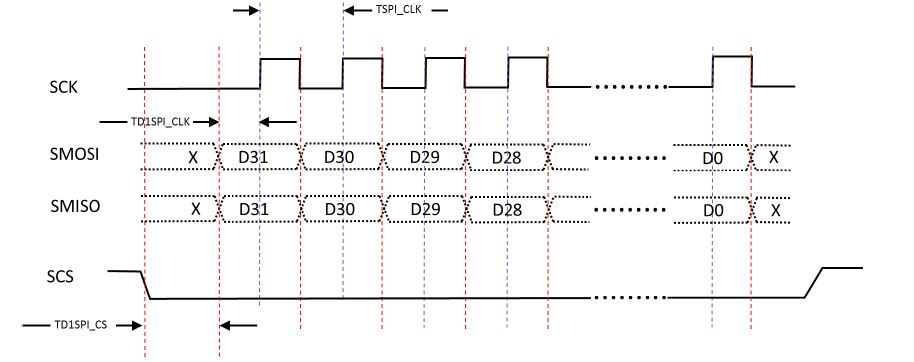
\includegraphics[width=0.9\textwidth]{SPI_Timing.jpg}
    \caption[]{SPI-Timing diagram) }
    \label{fig:SPI_Timing}
\end{figure}

The following definitions hold for the ASIC in use:


\begin{table}[H]

\caption[]{SPI Definitions}
    \label{tab:1}
    
  \begin{center}  
  \begin{tabular}{|r|l|}
  \hline
  \textbf{Name}  & \textbf{Definition} \\ \cline{1-2}
  
  \textbf{SCK} & SPI Serial Clock (output from Master) \\
  \textbf{SMOSI} &Master Output, Slave Input \\ 
  \textbf{SMISO} &Master Input, Slave Output\\
  \textbf{SCS} &Chip-Select (Active low, provided by Master)\\
  \hline
  
\end{tabular}
\end{center}
\end{table}


During one SPI communication cycle, the 32-bit word in the following configuration is sent to the ASIC serially on the SMOSI line.

\begin{table}[H]

\caption[]{Master to Slave serial bit-fields}
    \label{tab:2}
    
  \begin{center}  
  \begin{tabular}{|l|c|c|c|}
  \hline
  \textbf{Bit indices}  & 31 to 23  & 22 & 21 to 0\\ 
  \hline
  \textbf{Data Components} & SPI-Address & Read/Write Bit & SPI-Data \\
  \hline
  
\end{tabular}
\end{center}
\end{table}

The 32-bit word in the following configuration is sent from the ASIC serially on the SMISO line.

\begin{table}[H]

\caption[]{Slave to Master serial bit-fields}
    \label{tab:3}
    
  \begin{center}  
  \begin{tabular}{|l|c|c|c|}
  \hline
  \textbf{Bit indices}  & 31 to 23  & 22 & 21 to 0\\ 
  \hline
  \textbf{Data Components} & Meaningless & Meaningless & SPI-Data \\
  \hline
  
\end{tabular}
\end{center}
\end{table}
The SPI serial clock operates at minimum frequency of 1 kHz and at a maximum frequency of 5 MHz

\subsection{Design of digital hardware}
\label{sec:hardwaredesign}
\subsubsection{Introduction}

The language chosen for hardware generation is VHDL. The code was written and tested in the Libero SoC v11.7 integrated development environment. The company, which developed the environment is called Microsemi. They also provide pre-defined soft-cores such as the Core\_Uart which is used in the design. The hardware consists of a processing unit which takes commands from a computer, in the case of the CubeSat mission, this would be the on-board computer. The processing unit deciphers the input commands and interacts with the on-fabric memory as well as the ASIC. The testbenches are written in VHDL as well and the simulation software is called ModelSim and is automatically called from the Libero Interface and performs the simulation based on the specification in the testbench file. Many of the hardware components already existed in an undocumented form for the ASIC test board at PSI. The code for these components was written by Carla Brito from the company Efacec.


\subsubsection{Functional Block Diagram}

\begin{figure}[H]
    \centering
    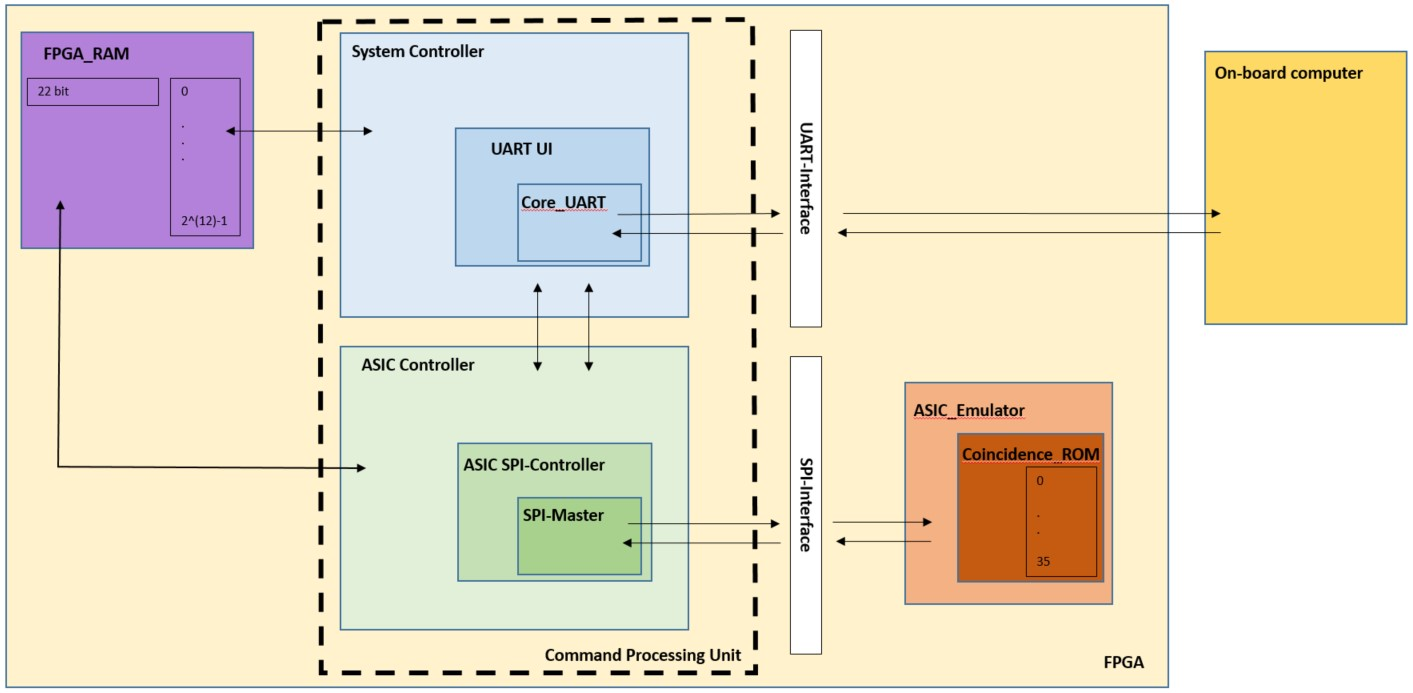
\includegraphics[width=0.9\textwidth]{Fucional_block.jpg}
    \caption[]{Functional block diagram implemented with VHDL logic) }
    \label{fig:Functional_block}
\end{figure}

The diagram above shall visualize the data flow on the FPGA architecture.

The diagram does not consider the connections and lines for the clock. In the Microsemi Libero environment, an on-board clock can be generated by connecting the output of the chip oscillator with a clock conditioning circuit, which generates the desired frequencies.
\newline

The memory on the FGPA is implemented using a RAM component. It stores data which is organized in the 22-bit format following the register size of the ASIC. It consists of 4096 readable and writeable addresses and therefore constitutes a memory of about 90 Kbit. The functionality and properties of the other blocks will be explained in their separate section later.
\newline

The oscillator in conjunction with the clock conditioning circuit generates a clock, which runs at a frequency of 20 MHz and is used for all the components except the ASIC emulator, who depends on the SPI-clock, which runs at a rate of 200 kHz.

\subsubsection{Bit-field logic of commands}
The half-duplex mode communication between the computer and the FPGA works via a serial UART interface utilizing 40-bit words.
\newline

Generally, the computer-to-FPGA commands have the following bit-field logic:

\begin{table}[H]

\caption[]{Computer-to-FPGA command constellation}
    \label{tab:4}
    
  \begin{center}  
  \begin{tabular}{|c|p{2cm}|p{2cm}|p{2.5cm}|p{2cm}|p{2cm}|}
  \hline
  \textbf{Bit indices forward}  & 39 to 36  & 35 & 34 & 33 to 22 & 21 to 0\\ 
  \hline
  \textbf{Data Components} & Command \newline Type & NO USE & Local Usage & Command Control Address & Data bits \\
  \hline
  
\end{tabular}
\end{center}
\end{table}

The FPGA-to-computer responses are in the following configuration:


\begin{table}[H]

\caption[]{FPGA-to-computer response constellation}
    \label{tab:5}
    
  \begin{center}  
  \begin{tabular}{|c|p{3cm}|p{3cm}|p{3cm}|}
  \hline
  \textbf{Bit indices response}  & 39 to 36  & 35 to 22 & 21 to 0 \\ 
  \hline
  \textbf{Data Components} & Command Type Response & Copy of computer-to-FPGA indices for verification & Data from memory or ASIC register data or copy of computer-to-FPGA indices for verification \\
  \hline
  
\end{tabular}
\end{center}
\end{table}

To write data to an ASIC register via the SPI-port, the following sequences must be sent via the UART port:


\begin{table}[H]

\caption[]{Write ASIC register command 1/2}
    \label{tab:6}
    
  \begin{center}  
  \begin{tabular}{|c|p{2cm}|p{2cm}|p{2.5cm}|p{2cm}|p{2cm}|}
  \hline
  \textbf{Bit indices}  & 39 to 36  & 35 & 34 & 33 to 22 & 21 to 0\\ 
  \hline
  \textbf{Values} & 0001  & 0 & 0 & 0x00A & Data bits \\
  \hline
  
\end{tabular}
\end{center}
\end{table}

\begin{table}[H]

\caption[]{Write ASIC register command 2/2}
    \label{tab:7}
    
  \begin{center}  
  \begin{tabular}{|c|p{1.5cm}|p{0.7cm}|p{1cm}|p{1cm}|p{1cm}|p{2cm}|p{2cm}|}
  \hline
  \textbf{Bit indices}  & 39 to 36  & 35 & 34 & 33 to 22 & 21 to 10 & 9 & 8 to 0\\ 
  \hline
  \textbf{Values} & 0001  & 0 & 0 & 0x009 & Meaningless, set to 0 & R/W bit, set to 1 & SPI register address \\
  \hline
  
\end{tabular}
\end{center}
\end{table}

To read data from an ASIC register via the SPI-port, the following sequences must be sent via the UART port:

\begin{table}[H]

\caption[]{Read ASIC register command 1/2}
    \label{tab:8}
    
  \begin{center}  
  \begin{tabular}{|c|p{1.5cm}|p{0.7cm}|p{1cm}|p{1cm}|p{1cm}|p{2cm}|p{2cm}|}
  \hline
  \textbf{Bit indices}  & 39 to 36  & 35 & 34 & 33 to 22 & 21 to 10 & 9 & 8 to 0\\ 
  \hline
  \textbf{Values} & 0001  & 0 & 0 & 0x009 & Meaningless, set to 0 & R/W bit, set to 0 & SPI register address \\
  \hline
  
\end{tabular}
\end{center}
\end{table}

\begin{table}[H]

\caption[]{Read ASIC register command 2/2}
    \label{tab:8}
    
  \begin{center}  
  \begin{tabular}{|c|p{1.5cm}|p{0.7cm}|p{1cm}|p{1cm}|p{3cm}|}
  \hline
  \textbf{Bit indices}  & 39 to 36  & 35 & 34 & 33 to 22 & 21 to 0 \\ 
  \hline
  \textbf{Values} & 0000  & 0 & 0 & 0x00D & Meaningless, set to 0  \\
  \hline
  
\end{tabular}
\end{center}
\end{table}

\subsection{System Description}
In this chapter, the individual blocks of the VHDL design are documented in detail.

\subsubsection{UART UI (User Interface)}
This component is responsible for several tasks. First, it converts the serial one line UART RX input into a parallel data line. At the same time, it is responsible for sending a desired output given as parallel register content via the serial UART TX port. For this reason, the sub-block Core UART is employed in this component. It is a native soft core, which means that it is synthesizable pre-written hardware that can be instantiated several times. This softcore is available on the SmartFusion2 as well as the ProASIC3 FPGAs. The core can receive one byte at a time via the serial UART RX port in the following fashion:

\begin{figure}[H]
    \centering
    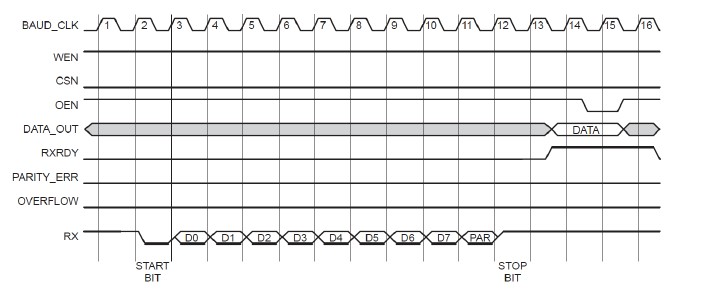
\includegraphics[width=0.89\textwidth]{UART_serial_rx.jpg}
    \caption[]{UART serial receive (\cite{UART}) }
    \label{fig:UART_serial_rx}
\end{figure}

Likewise, one byte at a time can be sent by putting the data at the DATA\_IN port of the Core and setting the WEN (write enable) to active low for at least one clock cycle

\begin{figure}[H]
    \centering
    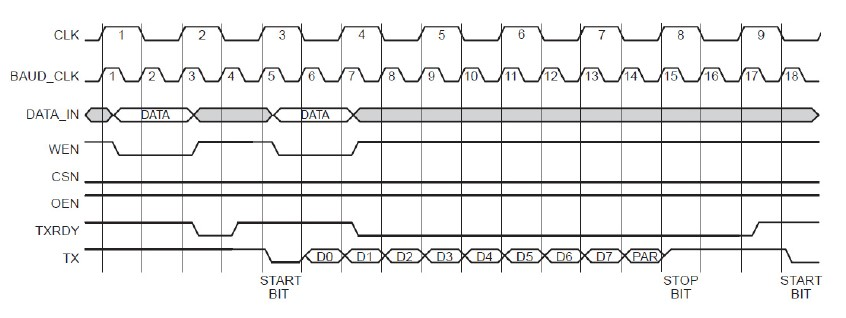
\includegraphics[width=0.89\textwidth]{UART_serial_TX.jpg}
    \caption[]{UART serial transmit (\cite{UART}) }
    \label{fig:UART_serial_TX}
\end{figure}
The Core is operating with the following UART parameters:


\begin{table}[H]

\caption[]{UART Core specifications}
    \label{tab:9}
    
  \begin{center}  
  \begin{tabular}{|r|l|}
  \hline
  \textbf{Parameter}  & \textbf{Value} \\ \cline{1-2}
  
  \textbf{Clock rate} & 20 MHz \\
  \textbf{Baud Rate [Hz]} & 460800\\ 
  \textbf{Baud Rate Adjust} & +0.712 \\
  \textbf{Bit Width} & 8\\
  \textbf{Active Chip Select} & Low \\
  \textbf{Enable Parity} & Yes \\
  \textbf{Parity Type} & Odd \\
  \hline
  
\end{tabular}
\end{center}
\end{table}


However, this is not everything that has to be done, since one command consists of 40 bits a total of 5 bytes need to be sent through the UART port. The UART UI therefore needs to keep track of how many bytes have already been received and re-construct the 40 bit-word by assembling 5 bytes together. Afterwards, the command data and command address must be separated and stored in their designated data lines to be processed by the System Controller, which is one hierarchy stage above the UART UI.

\begin{figure}[H]
    \centering
    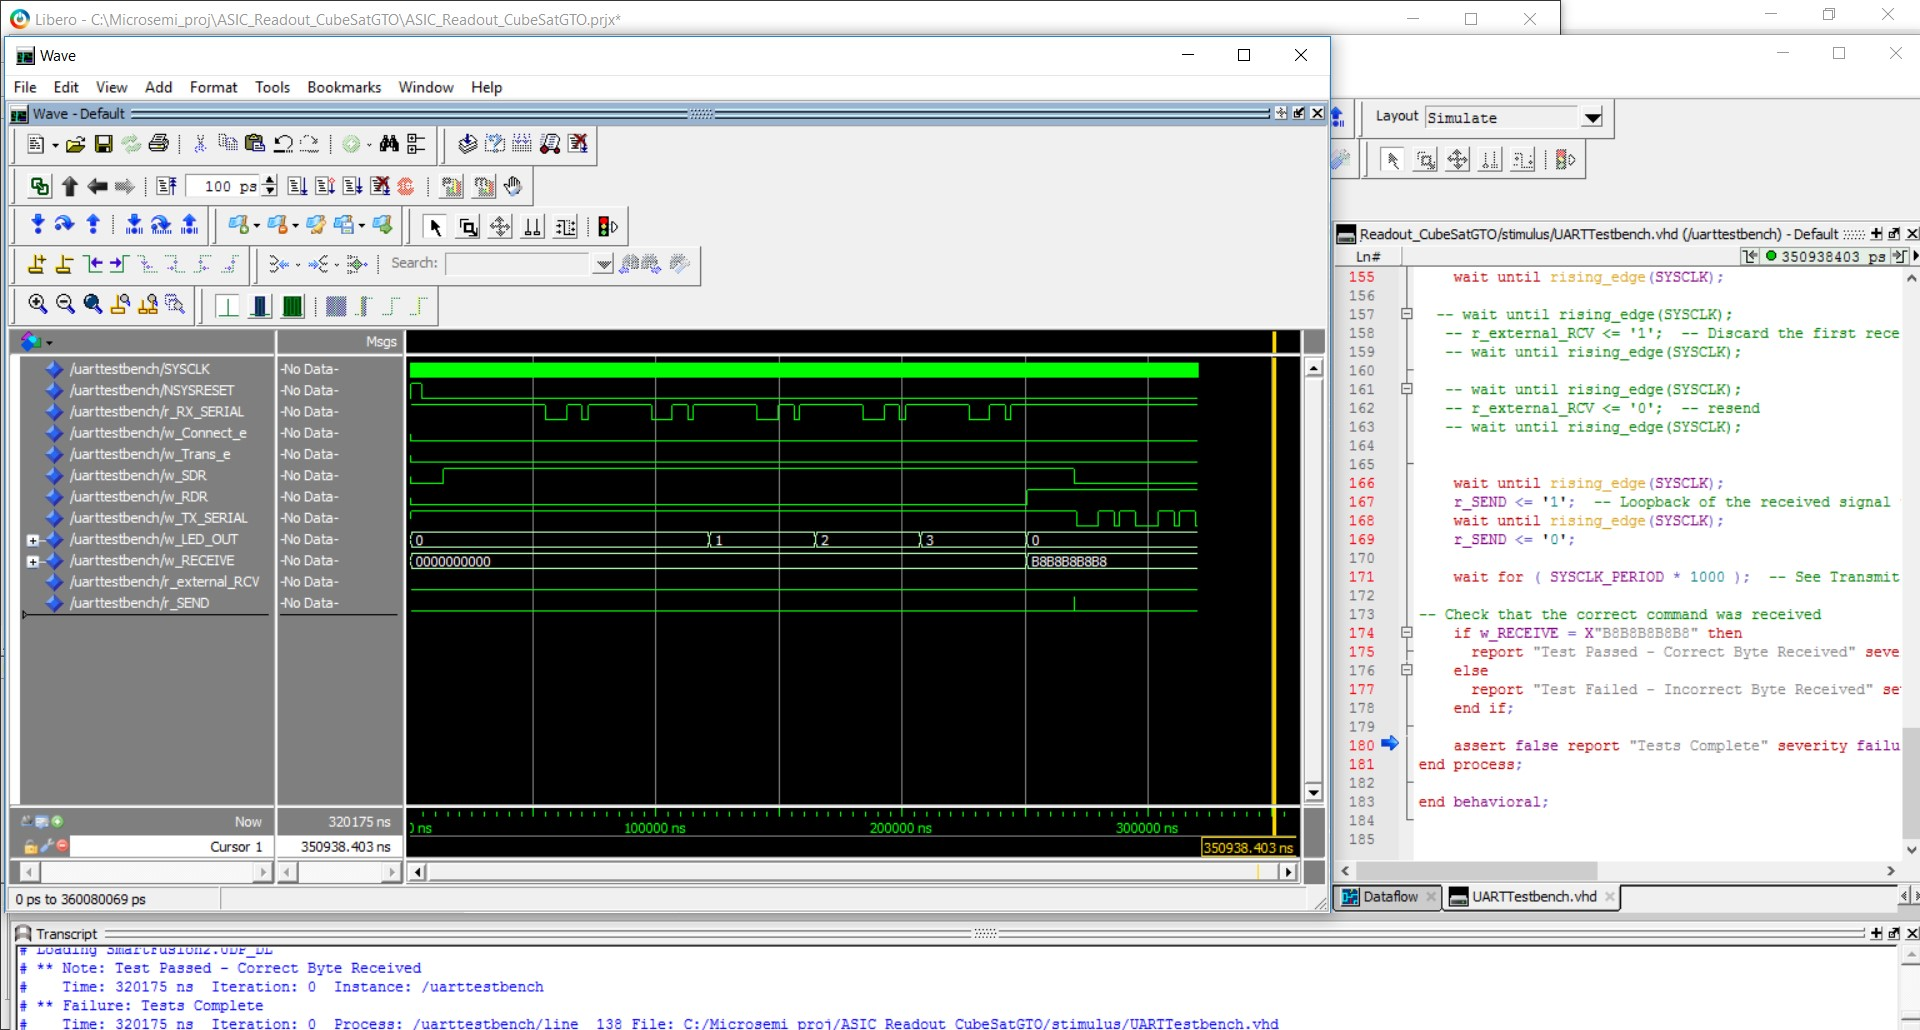
\includegraphics[width=0.89\textwidth]{UART_SIMULATE.jpg}
    \caption[]{UART Interface Test Bench and Simulation) }
    \label{fig:UART_SIMULATE}
\end{figure}

In the wave diagram above, the r\_RX\_SERIAL port depicts the UART input, that is instructed to serially send data to be received by the UART UI. The 40-bit word is successfully re-constructed and stored in the w\_RECEIVE register and via the r\_SEND signal, the serial UART transmit operation can be initiated and the result can be observed on the w\_TX\_SERIAL data line.
\subsubsection{System Controller}
The system controller is the main part of the command processing unit. It deciphers the instructions and controls the data flow accordingly. If instructed to read or write ASIC registers, it is responsible for the delivering of the command data as well as the command address to the ASIC Controller, which is the component that initiates the communication with the ASIC. Furthermore, after each successfully received instruction, the system controller builds the appropriate response and sends it automatically back to the computer via the serial UART transmit port. If instructed to read memory, one command is enough to either read or write a memory address specified in the command address portion of the instruction and immediately send back the data in the memory address to the computer. Due to its relative complexity, a diagram of its state machine has been created.

\begin{figure}[H]
    \centering
    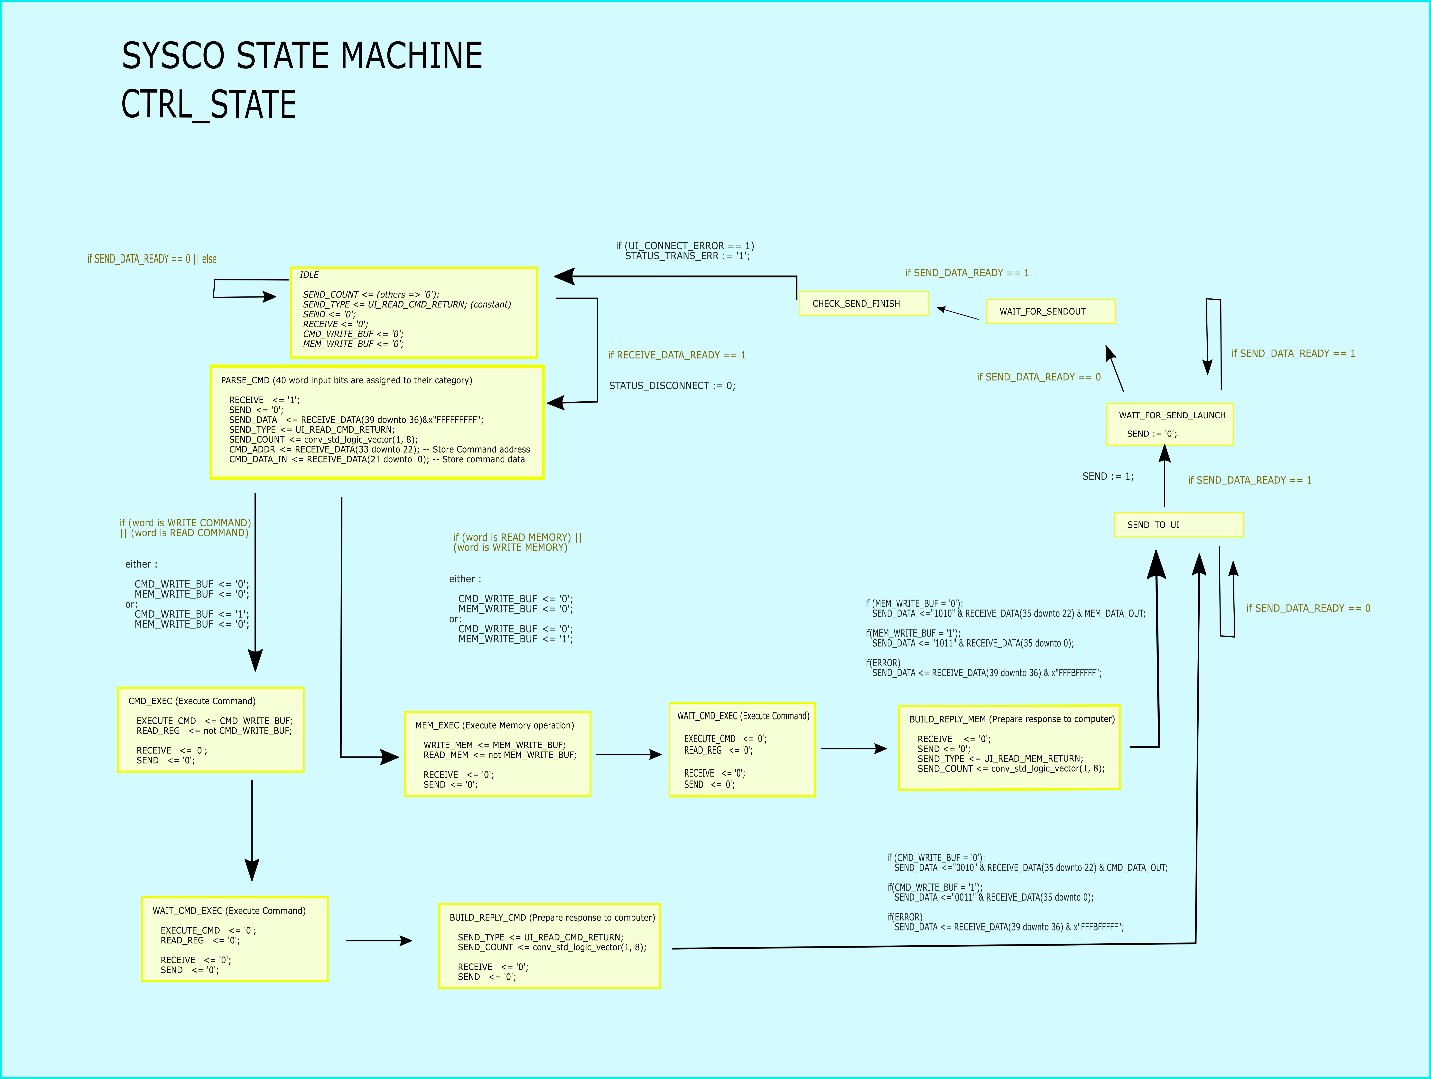
\includegraphics[width=0.89\textwidth]{SYSCO_StateMachine.jpg}
    \caption[]{State machine of the system controller) }
    \label{fig:SYSCO}
\end{figure}
Another testbench has been written to simulate the System Controller design.

\begin{figure}[H]
    \centering
    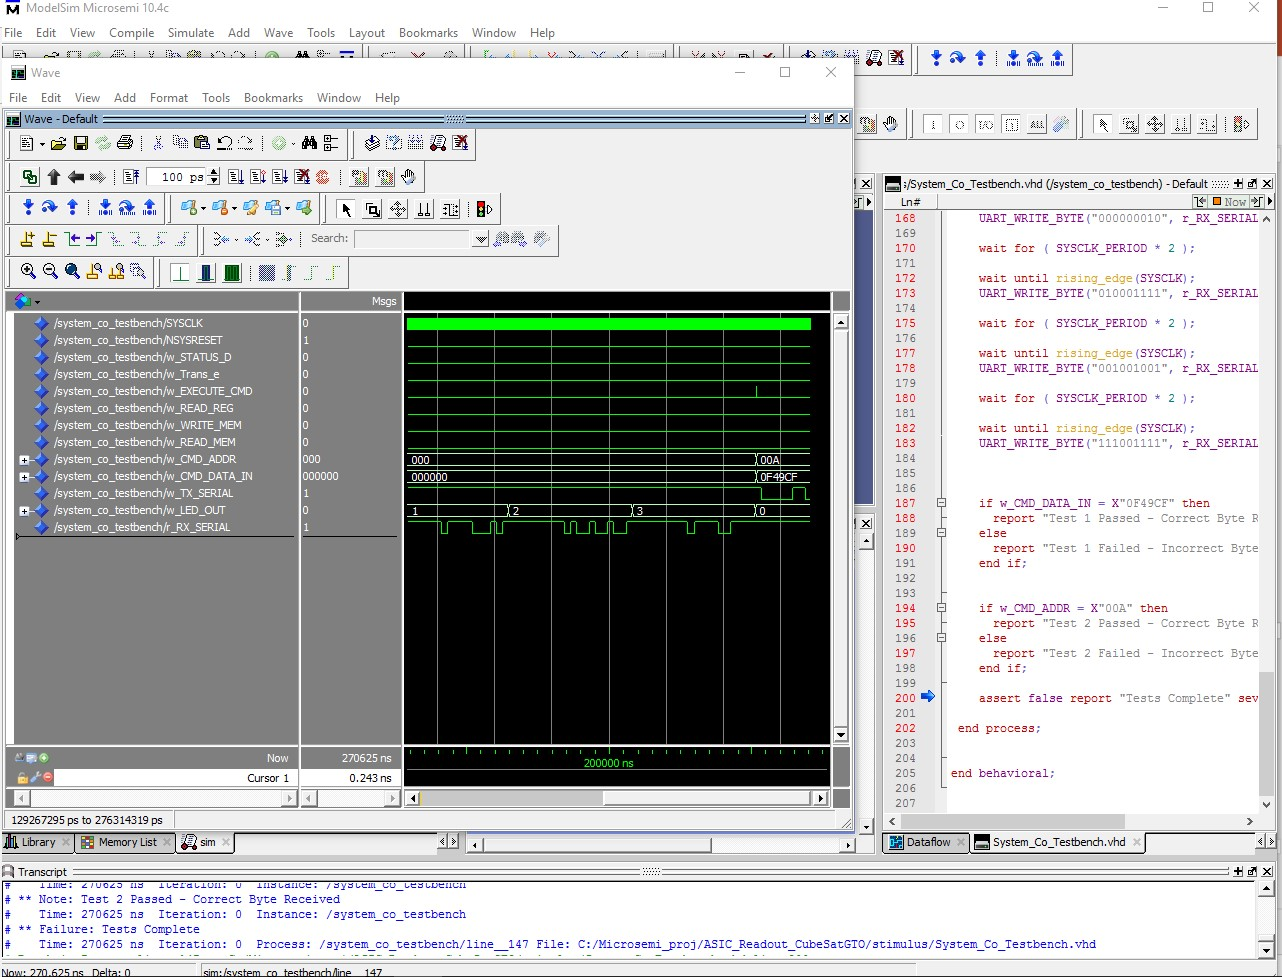
\includegraphics[width=0.8\textwidth]{SYSCO_Simulate.jpg}
    \caption[]{Simulation of the System Controller }
    \label{fig:SYSCO_Sim}
\end{figure}

In this example, like the one described for the UART UI, an instruction is sent through the r\_RX\_SERIAL port, the System Controller parses the input and stores the command address and command data in w\_CMD\_ADDR and w\_CMD\_DATA\_IN respectively. It also interprets the command as a write command to the ASIC and therefore sets the w\_EXECUTE\_CMD for the ASIC Controller to 1 for one cycle.

\subsubsection{ASIC Controller and SPI-Master}
The ASIC Controller is the second of two main components for the command and communication processing. It is mainly responsible for initiation communication with the ASIC by establishing a link using the SPI protocol. An illustration of its state machine has been created. 

\begin{figure}[H]
    \centering
    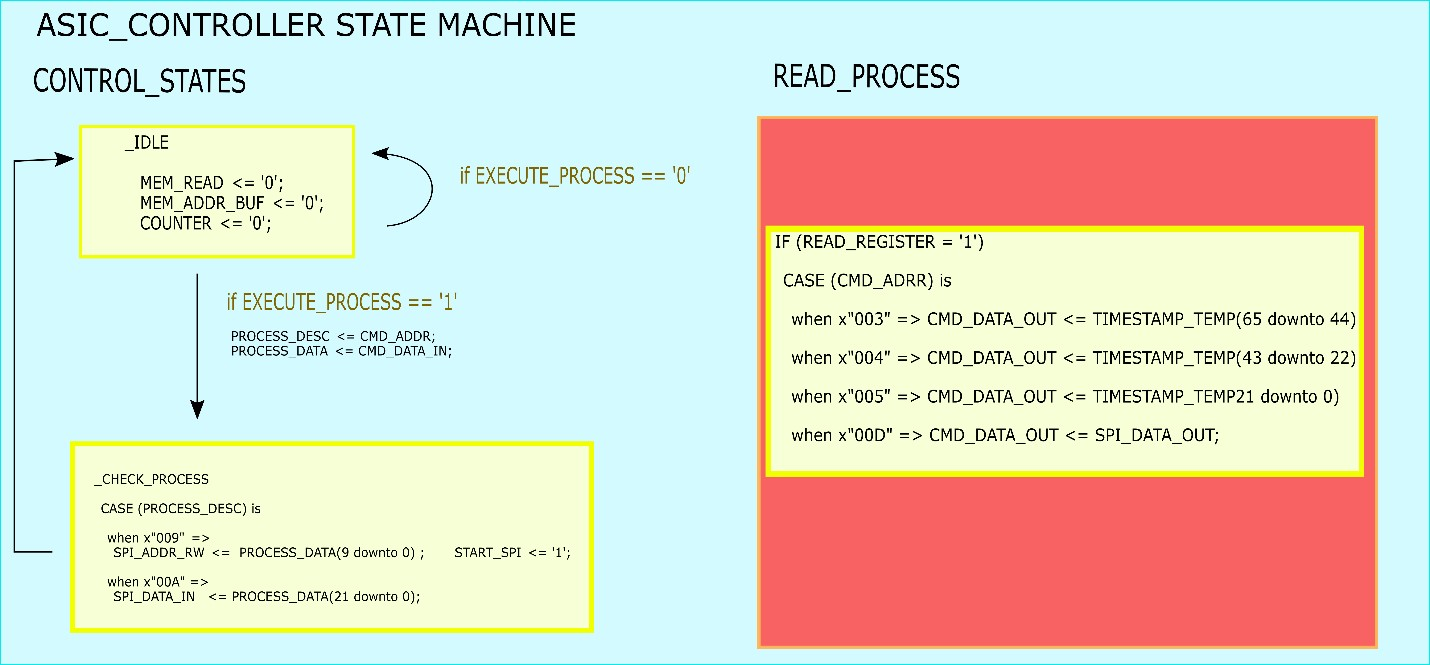
\includegraphics[width=0.89\textwidth]{ASIC_Controller_STATEMACHINE.jpg}
    \caption[]{ASIC Controller State Machine}
    \label{fig:ASIC_CON_STATE}
\end{figure}

After the System Controller has parsed the input, it will either send an impulse on the EXECUTE\_PROCESS or the READ\_REGISTER line, the former defines the data or the address of the registers of the ASIC that should be read or written through the CMD\_ADDR and CMD\_DATA\_IN registers.

One hierarchy stage below, the SPI Control Unit is affiliated in the design. The SPI Control Unit is in turn one stage above the SPI-Master and is mainly responsible for implementing system resets for the SPI port that are sent from anywhere in the command processing unit, it can overwrite the SPI clock and the data lines if a reset is requested. Its state machine diagram can be found below. 

\begin{figure}[H]
    \centering
    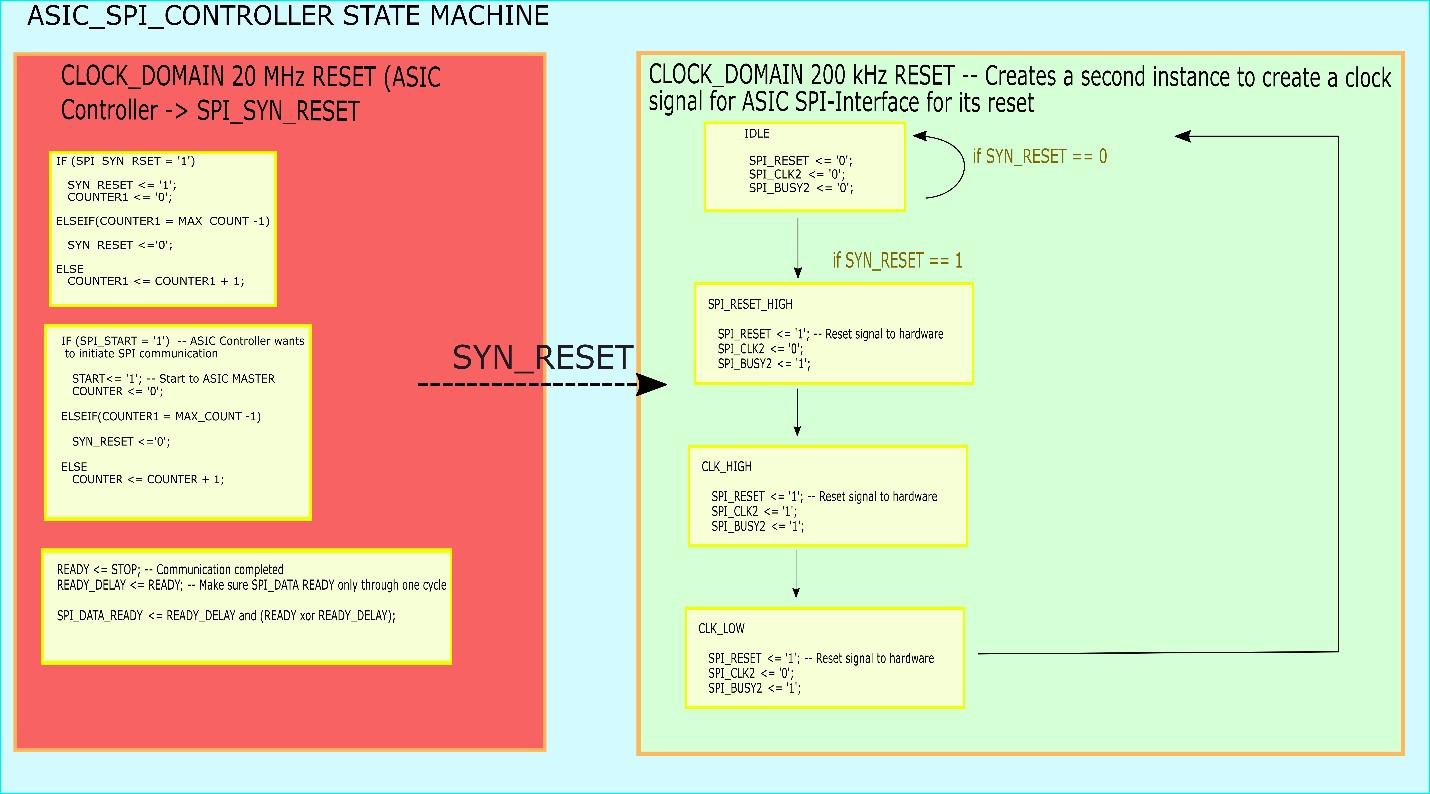
\includegraphics[width=0.8\textwidth]{SPI_control.jpg}
    \caption[]{SPI Control Unit State machine, clock domains and non-sequential logic part}
    \label{fig:ASIC_SPI_STATE}
\end{figure}

And finally, the SPI Master is added one stage below whose outputs and inputs are directly connected to the digital hardware interface of the ASIC. The SPI master combines the SPI-Address the Read/Write Mask bit and the SPI-Data to a 32-bit register which is serially transmitted over the SPI interface if the ASIC Controller initiates an SPI transaction. The state machine of the SPI-Master is depicted in the figure below.

\begin{figure}[H]
    \centering
    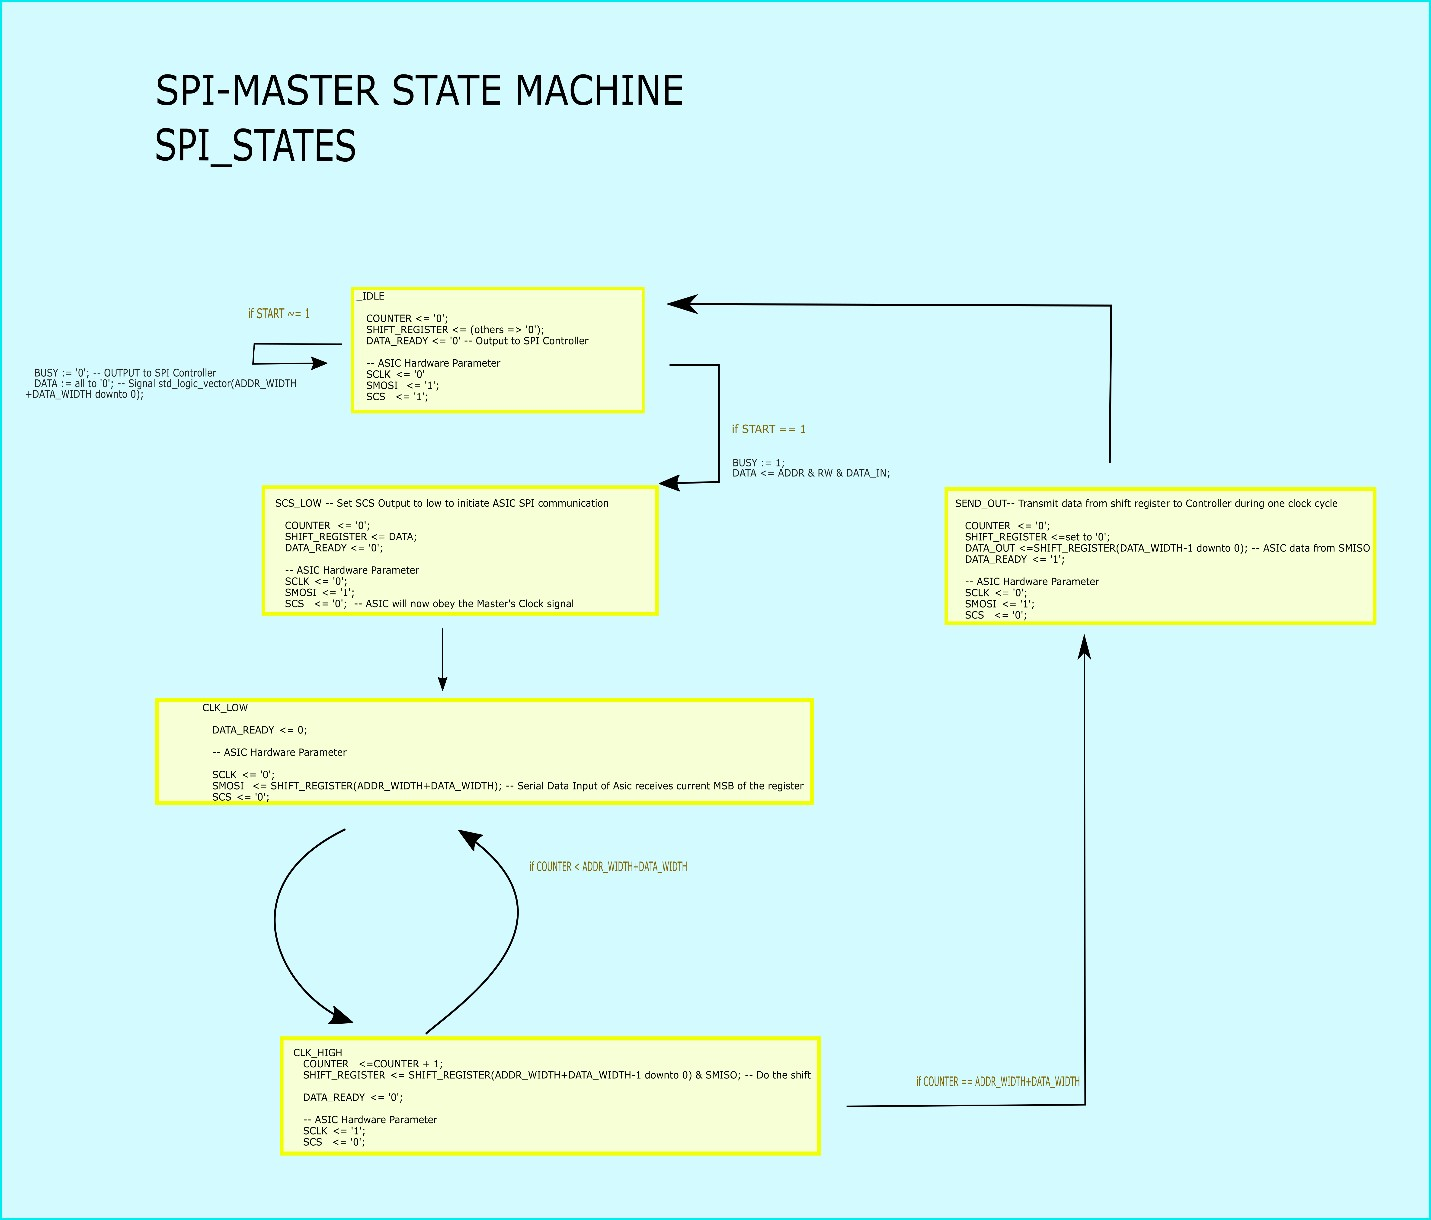
\includegraphics[width=0.8\textwidth]{SPI_master.jpg}
    \caption[]{SPI-Master State Machine}
    \label{fig:SPI_master}
\end{figure}

The hardware instantiation in the Libero software without the ASIC emulator is depicted in the figure below.

\begin{figure}[H]
    \centering
    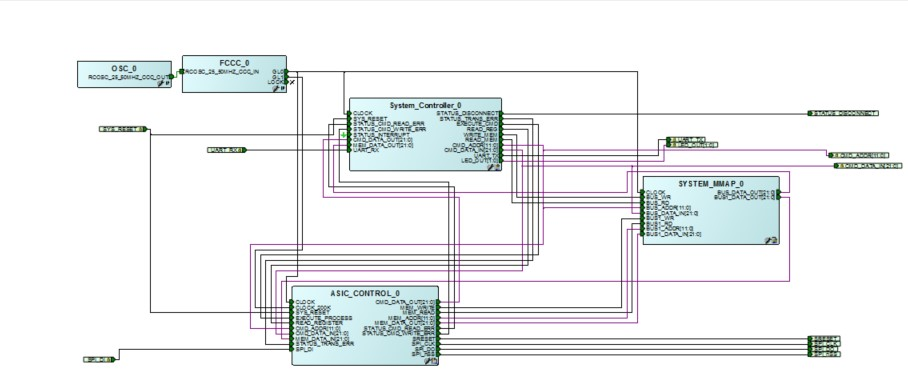
\includegraphics[width=\textwidth]{Design_Instantiate.jpg}
    \caption[]{Hardware Block-Diagram of Readout design, instantiation in Libero SoC}
    \label{fig:Instantiate}
\end{figure}

\subsection{ASIC emulator}
The price for the IDE3466 ASIC is beyond what was affordable and due to that unfortunate test, there was no physical device to be tested in the scope of this projects. To test the programmed hardware and to expand the read-out electronic design in a future project, the hardware code for an emulation of a simplified ASIC was developed. It implements an SPI-slave that can conduct a full-duplex communication with the SPI-Master and the rest of the read-out design. 
\newline 

The counter registers of the coincidence sub-unit were implemented using a ROM architecture. The register addresses for the counters match the ones specified in the ASIC data sheet. This allows the commands to be in the same configuration as in the real case. 
\newline

Its state machine of the SPI slave is very like the one of the Master with the exception that its data output is only meaningful as soon as the register address has completely been read by the emulator. On the other hand, it is possible to specify the address that should be read and receive its content within the same transaction. 


\begin{figure}[H]
    \centering
    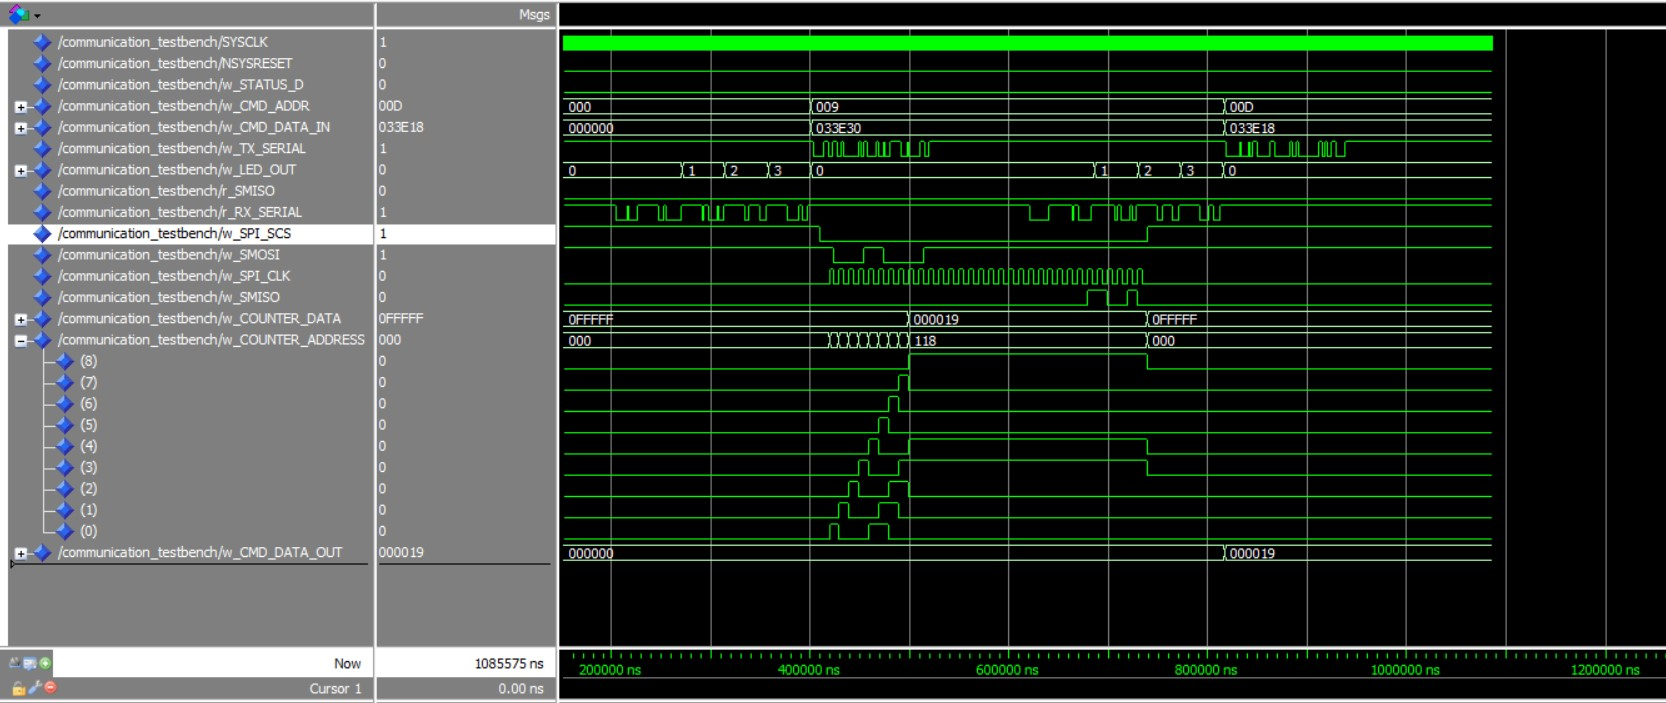
\includegraphics[width=\textwidth]{Simulation_design.jpg}
    \caption[]{Simulation of the design}
    \label{fig:Simulation}
\end{figure}

The simulation above depicts the behavior of the architecture when an ASIC register is read. As soon as the first command is sent through the UART port, the instruction is deciphered and the SPI-protocol begins, the ASIC emulator on the hardware interface is selected and the signals w\_SPI\_CLK and w\_SMOSI are used for specifying the address in the ASIC. The emulator internally uses a shift register whose value can be observed in w\_COUNTER\_ADDRESS. Towards the end of the process, on the SMISO line, the value of the specified register is sent back to the readout design and stored in w\_CMD\_DATA\_OUT, which is directly connected to the UART UI, which sends it to the computer via the w\_TX\_SERIAl port in the configuration specified in (see sec. \ref{sec:hardwaredesign}).

\subsection{Implementation on FPGA}
The design was tested on the Microsemi SmartFusion2 M2S050 FPGA using the Starter Kit development board.
\newline

The SmartFusion2 M2S050 also includes a Microcontroller Subsystem (MCSS) on its chip, which is not in use however, due to the lower radiation tolerance of software components compared to the fabric hardware.
\newline

For the actual read-out board, a different FPGA has been considered a superior choice over the SmartFusion2 device. The ProASIC3 A3P1000 does not come with the superfluous MCSS. The implementation of the code is not expected to cause any problems, the utilized softcores are available on the ProASIC3 as well and the same development environment supports the product.


